\chapter{Literature Review}

\section{Cardiac Diffusion MRI}

Magnetic Resonance Imaging (MRI) is the imaging method that was used to acquire the data on which our results are based. It is non-invasive and especially adapted to soft-tissues. \cite{bakermans2008} We will explain briefly how it works and what information it gives us.

\subsection{Physics of MRI}

Magnetic Resonance acquisitions rely on the physical properties of the body, and more specifically the most abundant nucleus which is hydrogen (H). Indeed water molecules ($H_2O$, therefore 2 nucleus of hydrogen in each molecule) represent more than 60\% of the entire body composition. This hydrogen nucleus H consists of 1 proton and 1 electron (which is not important in this case) of opposite electrical charge. The proton spins around itself and therefore creates a magnetic moment which makes the nucleus behave like a magnet from the outside world.
\begin{figure}
    \centering
    \begin{subfigure}[t]{.30\textwidth}
        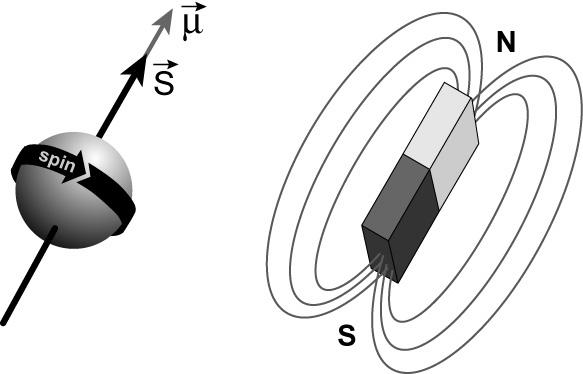
\includegraphics[width=\textwidth]{figures/hydrogen_magnet}
        \caption{The hydrogen proton behaves like a magnetic dipole}
        \label{fig:hydrogen_magnet}
    \end{subfigure}
    \begin{subfigure}[t]{.68\textwidth}
        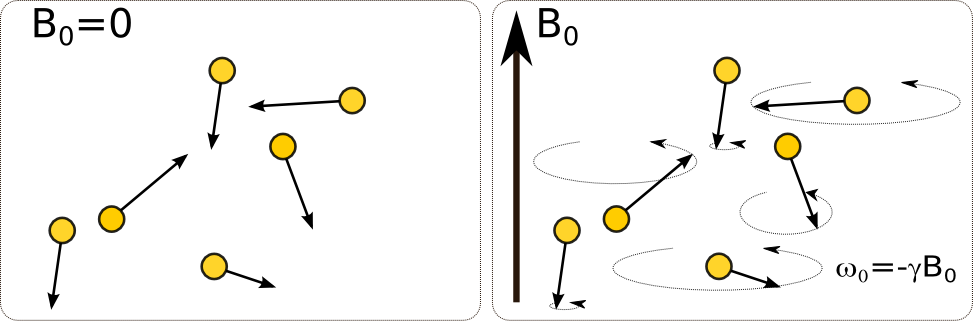
\includegraphics[width=\textwidth]{figures/Precession_Larmor_2}
        \caption{The Larmor precession when an exterior magnetic field is present - \cite{hydrogen}}
        \label{fig:larmor_precession}
    \end{subfigure}
    \caption{Magnetic behavior of the hydrogen nucleus}
    \label{fig:hydrogen}
\end{figure}

Applying an external magnetic field $\mathbf{B_0}$ leads to a precession around the direction of $\mathbf{B_0}$ of the nuclear magnetic moment of the nucleus. Its magnetic moment will have a characteristic Larmor frequency $\omega_0$. All the magnetic moments of the nuclei in a specific region will average out to a net magnetization vector $\mathbf{M_0}$ aligned with $\mathbf{B_0}$. Though it is important to note that all protons will have a different phase and that the precession is asynchronous between all protons, as shown in \ref{fig:larmor_precession}.\\
Then the idea is to apply a secondary and much less intense magnetic field $\mathbf{B_1}$, with $||\mathbf{B_1}|| \simeq 10^{-6}||\mathbf{B_0}||$ in a direction in the plane orthogonal to the direction of $\mathbf{B_0}$, rotating around the direction of $\mathbf{B_0}$ with the Larmor frequency $\omega_0$ to bring the nuclei to resonance and out of their equilibrium, ie into an excited state \ref{fig:spin_excitation}. A torque will indeed be applied to the magnetic moment of the nucleus, coming from the Lorentz force: $\tau = \mathbf{M} \times \mathbf{B_1}$ where $\mathbf{M}$ is the magnetic moment of the nucleus. This can be achieved by transmitting radio frequency (RF) pulses. Then all nucleus motion will be synchrone and in phase.\\
\begin{figure}[h!]
    \centering
    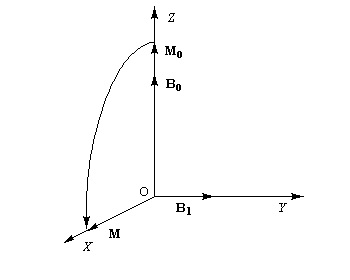
\includegraphics[width=.5\textwidth]{figures/spin_excitation}
    \caption{Torque effect on the magnetic moment of the proton $\mathbf{M}$ when applying an extra magnetic field $\mathbf{B_1}$}
    \label{fig:spin_excitation}
\end{figure}
\\
Once the impulse stops, the protons will go back to non-coordinated state by leaving their excited state and in that process emitting another magnetic signal (weak compared to $\mathbf{B_0}$) that will be analyzed and specific to each proton. This information will be used to understand the distribution of the orientation of the magnetic moments in the environment.\\
Indeed, the motion of water molecule is constrained by its environment (tissue, nerves...), which is why the measurement of this anisotropic diffusion reveals structural properties of the tissue we are interested in.

\subsection{At the service of Imaging}

Once the nuclei are in its excited state, its relaxation \ref{fig:spin_relaxation} and the outcome magnetization vector in the $(x, y)$ plane $\mathbf{M_{x, y}}$ induces a current recorded by a RF receiving coil.
\begin{figure}[h!]
    \centering
    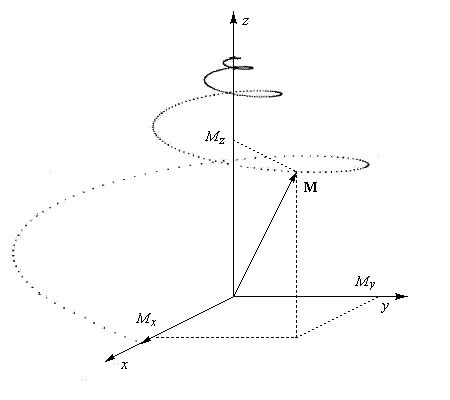
\includegraphics[width=.5\textwidth]{figures/spin_relaxation}
    \caption{Relaxation of the magnetic spin after the magnetic pulse $\mathbf{B_1}$ stops}
    \label{fig:spin_relaxation}
\end{figure}
\\
This is the signal that is measured in a MR experiment and that will be used to acquire the data.\\
For acquisitions in 2D or 3D there are gradient applied to the RF pulse depending on the location, so that the receiving coil can differentiate more easily depending on this modulation. Typically in 2D for a slice they use frequency and phase encoding for the 2 degrees of freedom. In 3D slice selection is accomplished via a linear magnetic gradient, so that the main exterior magnetic field $\mathbf{B_0}(z)$ is different for each slice and leads to different Larmor values for each value of $z$.\\
In our case all MRI are acquired ex-vivo, which means that the acquisition process is more simple as the subject is perfectly still and several acquisitions can be performed without having to worry about the subject's motion. More advanced techniques are invoked such as FLASH imaging to solve these extra requirements.

\section{Diffusion Tensor Imaging}

Magnetic resonance diffusion tensor imaging (DTI) is a method based on MRI and the diffusion mechanism of water molecules to assess the direction of fibers from the anisotropic property of the diffusion of these molecules in a structure that contains boundaries.\\

\subsection{Physical diffusion property of molecules}

In general the DTI signal is based on the proton of the hydrogen nucleus present in water molecules.\\
In a non-restrictive volume, the motion of molecules also called Brownian motion has a Gaussian distribution at equilibrium that is linked to the temperature of the environment and other properties of this environment. This Gaussian distribution will be deviated in the presence of physical barriers that will decrease the diffusivity. Indeed molecules' motion will be hindered in the direction perpendicular to the obstacles. When barriers are present the diffusion will change from isotropic to anisotropic. If we look at a free water molecule, its diffusion would be in the shape of a sphere whereas with boundaries the diffusion of the same water molecule would be more of an ellipsoid with principal direction orthogonal to the boundary.

\subsection{Applied to diffusion weighted imaging} \label{dw_imaging}

Two short and intense successive pulsed field gradients (PFGs) are applied to the region of interest. The first makes protons have a precession phase proportional to their position along the direction of the gradient. Then a second one is applied with the exact opposite direction so that molecules that didn't move will have a precession phase null whereas those that moved will have a precession phase proportional to their motion in the direction of the PFG. Here we talk about single water molecules but in reality we are considering distribution of water molecules, and for unbounded water molecules the distribution will be centered around a null motion whereas bounded ones will have a motion distribution centered around the direction orthogonal to the main boundary.\\
\begin{figure}[h!]
    \centering
    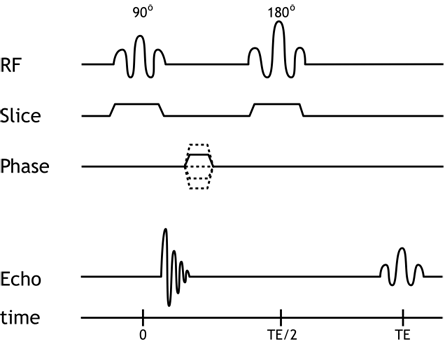
\includegraphics[width=.5\textwidth]{figures/pgse}
    \caption{Pulse Gradient Spin Echo (PGSE) sequence}
    \label{fig:pgse}
\end{figure}
\\
The acquisition sequence, also called Pulse Gradient Spin Echo (PGSE) sequence, can be described as follows: \cite{assemlal2011recent}
\begin{enumerate}
    \item A first PFG is applied in a direction orthogonal to the main magnetic field $\mathbf{B_0}$ for $t \in [0, \delta]$.\\
    This will have the effect to flip the nuclear spins in the direction of the impulse
    \item Once the impulse is over, the magnetic moment of the nuclei will start dephasing as they will start rotating around the direction of $\mathbf{B_0}$, each of them with their specific frequency related to the strength of the magnetic field at their specific location
    \item After a diffusion time $t = \Delta$, another PFG is applied and this time with a direction opposite to the first impulse for $t \in [\Delta, \Delta + \delta]$, which will refocus the spin phases
    \item Finally at the echo time $t = TE$, the diffusion signal is received by the scanner coil with a loss proportional to the displacement of water molecule during this process. It is the information given by the displacement that will give us useful insight regarding the micro structure of the studied environment.
\end{enumerate}

The equation of Nuclear Magnetic Resonance (NMR) was given by Stejskal and Tanner in 1965: it quantifies the decrease in signal intensity and relates it with the apparent diffusion coefficient $\mathbf{D}$.\\
Let $\mathbf{G}(t) = \Big(H\big(t - t_1\big) - H\big(t - (t_1 + \delta)\big)\Big)\mathbf{u} + \Big(H\big(t - t_2\big) - H\big(t - (t_2 + \delta)\big)\Big) \mathbf{v}$ \\
where $\mathbf{u}, \mathbf{v}$ are unit vectors in the direction of the applied gradients, and $H(t)$ the Heaviside function at a given time $t$. Basically this function is the exact mathematical description of the PGSE sequence. Then we get the following Stejskal and Tanner equation:

\begin{equation} \label{eq:tanner}
\frac{S(TE)}{S_0} = \exp\Big({-\gamma^2G^2\delta^2(\Delta - \frac{\delta}{3})\mathbf{G}^T\mathbf{D}\mathbf{G}\Big)} = \exp (-b \times \mathbf{D})
\end{equation}

with the following:

\begin{itemize}
    \item $\gamma$: gyromagnetic ratio, constant specific to each molecule
    \item $G$: PFG strength
    \item $\delta$: duration of the pulse
    \item $\Delta$: time between 2 pulses
    \item $\mathbf{D}$: apparent diffusion coefficient
    \item $b$ factor suggested by LeBihan: $b = \gamma^2G^2\delta^2(\Delta - \frac{\delta}{3})||\mathbf{G}||^2$
\end{itemize}

\subsection{To get a diffusion tensor matrix}

Diffusion anisotropy can be described mathematically by a 3x3 diffusion tensor:
\begin{equation}
    \mathbb{D} = \begin{pmatrix}
    D_{xx} & D_{xy} & D_{xz} \\
    D_{yx} & D_{yy} & D_{yz} \\
    D_{zx} & D_{zy} & D_{zz}
    \end{pmatrix}
\end{equation}

with $D_{ij}$ the apparent diffusion coefficient (ADC) in direction $(i, j)$. In an environment dominated by water molecules, principles of thermodynamics dictate that $\mathbb{D}$ is symmetric, which means that $D_{ij} = D_{ji}$.\\
In conclusion we need at least 6 independent gradient directions to determine all 6 degrees of freedom in this matrix. In practice 7 directions are used to get more accurate results, along with a non-weighted measurement for normalization.\\
The values that we analyze most frequently are ADC and fracional anisotropy (FA):
\begin{equation}
    ADC = \frac{tr{\mathbb{D}}}{3} = \frac{\lambda_1 + \lambda_2 + \lambda_3}{3}
\end{equation}
\begin{equation}
    FA = \sqrt{\frac{(\lambda_1 - \lambda_2)^2 + (\lambda_2 - \lambda_3)^2 + (\lambda_3 - \lambda_1)^2}{\lambda_1^2 + \lambda_2^2 + \lambda_3^2}}
\end{equation}

\section{Heart fiber geometry}

From the 1970s, papers have shown how myofibers in the left ventricule (LV) are aligned in a way that they form helical curves \cite{savadjiev2012heart}. This alignment has proved to be optimal for its mechanical function. Heart fibers stay locally packed together and almost parallel to each other, although they are bundled into a special surface: a generalized helicoid \cite{blair1978generalization}. This is a minimal surface that maintains this property through the whole beat cycle. The bundle of myofibers in generalized helicoids is their characteristic orientation through the heart wall.

\subsection{The Generalized Helicoid Model (GHM)}

We will introduce a local frame field $\mathbf{f}_1,\mathbf{f}_2,\mathbf{f}_3 : \mathbb{R}^3 \to \mathbb{R}^3$ that will allow us to describre more easily the GHM. In this description,
\begin{itemize}
    \item $\mathbf{f}_1$: local orientation of the fiber
    \item $\mathbf{f}_3$: local heart wall normal
    \item $\mathbf{f}_2 = \mathbf{f}_3 \times \mathbf{f}_1$: cross product of the other 2 to get a right-handed orthogonal coordinate frame field
\end{itemize}

\begin{figure}[h!]
    \centering
    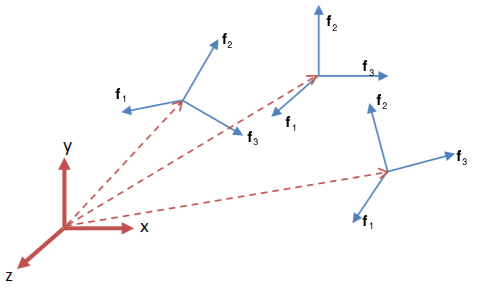
\includegraphics[width=.5\textwidth]{figures/frame_fields}
    \caption{Examples of possible local frame fields in a world coordinate system $(x, y, z)$}
    \label{fig:frame_fields}
\end{figure}

In the GHM model the fiber orientation is expressed at each point $(x, y, z) \in \mathbb{R}^3$ by the function:
\begin{equation}
\theta (x, y, z) = \arctan \Bigg( \frac{K_Tx + K_Ny}{1 + K_Nx - K_Ty} \Bigg) + K_Bz
\end{equation}
where $\theta$ is the angle $\angle (\overrightarrow{x}, \overrightarrow{y})$
\begin{itemize}
    \item $K_T$ causes bending in the tangent direction to the fiber
    \item $K_N$ makes fibers fan out, away from each other, in the $\mathbf{f}_2$ direction
    \item $K_B$ copies rotated versions of the fiber in planes parallel to the original $(x, y)$ plane, ie in the direction orthogonal to the heart wall
\end{itemize}
In general those values describe the amount of change in fiber orientation when going in each of the direction: tangential, orthogonal and out of plane.\\
Analyses of these parameters on different species has shown on the entire heart volume \cite{savadjiev2012heart} that the GHM fits with small values of $K_T$ and $K_N$ and high values of $K_B$. This validates the helicoidal model approach and the characteristic of the helix angle in the heart myofiber structure.

\subsection{The Maurer-Cartan form}

The Maurer-Cartan form operator has proved useful in measuring the differential structure of a manifold, and the theory of moving frame has shown good results in the modeling of the heart fiber geometry \cite{pami2015}. The main idea is to apply the theory of moving frames but reverse it: tuning the Maurer-Cartan connection forms can enable us to generate manifolds based on assumptions on the structure that represent in the best way possible the actual heart fiber structure. This approach can be executed by using different fitting methods.

\subsubsection{Theory of moving frames}

We utilize the framework described in \cite{de1990ventricular} to describe the geometry of fiber orientation in the heart wall via rotations of a frame field that is fit to the diffusion MRI data. \\
Let a point $\mathbf{x} = \sum_i{x_i\mathbf{e_i}} \in \mathbb{R}^3$ be expressed in terms of $(\mathbf{e_1}, \mathbf{e_2}, \mathbf{e_3})$, the natural basis for $\mathbb{R}^3$. \\
We define a right-handed orthonormal frame field $\mathbf{f}_1,\mathbf{f}_2,\mathbf{f}_3 : \mathbb{R}^3 \to \mathbb{R}^3$. \\ 
Each frame axis can be expressed by the rigid rotation $f_i = \sum_i{a_{i,j}\mathbf{e}_j}$, where $\mathbf{A} = {a_{i,j}} \in \mathbb{R}^{3 \times 3}$ is a differentiable attitude matrix such that $\mathbf{A}^{-1} = \mathbf{A}^T$. \\
Treating $\mathbf{f}_i$ and $\mathbf{e}_j$ as symbols, we can write:
\begin{equation}
\begin{bmatrix}
    \mathbf{f}_1 \\
    \mathbf{f}_2 \\
    \mathbf{f}_3
\end{bmatrix} = \mathbf{A} \times \begin{bmatrix}
    \mathbf{e}_1 \\
    \mathbf{e}_2 \\
    \mathbf{e}_3
\end{bmatrix}
\end{equation}

Since each $\mathbf{e}_i$ is constant, the differential geometry of the frame field is completely characterized by $\mathbf{A}$. Taking the exterior derivative on both sides, we have:
\begin{equation} \label{eq:1}
\begin{split}
    \partial \begin{bmatrix}
                \mathbf{f}_1 \\
                \mathbf{f}_2 \\
                \mathbf{f}_3
            \end{bmatrix} &= (\partial \mathbf{A})\mathbf{A}^{-1}  \begin{bmatrix}
                \mathbf{f}_1 \\
                \mathbf{f}_2 \\
                \mathbf{f}_3
            \end{bmatrix} \\
            &= \mathbf{C}
            \begin{bmatrix}
                \mathbf{f}_1 \\
                \mathbf{f}_2 \\
                \mathbf{f}_3
            \end{bmatrix}
\end{split}
\end{equation}
where $\partial$ denotes the exterior derivative, and $\mathbf{C} = (\partial \mathbf{A}) \mathbf{A}^{-1} = (c_{i,j}) \in \mathbb{R}^{3 \times 3}$ is the Maurer-Cartan matrix of connection forms $(c_{i,j})$. \\
Writing $\mathbf{f}_i$ as symbols, \ref{eq:1} is to be understood as $\partial \mathbf{f}_i = \sum_j{c_{i,j}\mathbf{f}_j}$. \\
The Maurer-Cartan matrix is skew symmetric with zeros as diagonal entries so there are at most 3 independent, non-zero 1-forms: $c_{1,2}$, $c_{1,3}$, and $c_{2,3}$. \\
\begin{equation}
    \mathbf{C} = \begin{pmatrix}
    0 & c_{1,2} & c_{1,3} \\
    -c_{1,2} & 0 & c_{2,3} \\
    -c_{1,3} & -c_{2,3} & 0
    \end{pmatrix}
\end{equation}
1-forms operate on tangent vectors through contraction, written as $\partial \omega \langle \boldsymbol{\upsilon} \rangle \in \mathbb{R}$ for a general 1-form $\partial \omega = \sum_i{\omega_i \mathbf{e_i}}$ and tangent vector $\boldsymbol{\upsilon} \in \mathbb{R}^3$, which yields:
\begin{equation}
\begin{split}
    \partial \omega \langle \boldsymbol{\upsilon} \rangle &= \sum_i{\omega_i \partial \mathbf{e_i}} \big{\langle} \sum_j{\upsilon_j \mathbf{e_j}} \big{\rangle} \\
    &= \sum_i{\omega_i \upsilon_i}
\end{split}
\end{equation} since $\partial \mathbf{e_i} \langle \mathbf{e_j} \rangle = \delta_{i,j}$, where $\delta_{i,j}$ is the Kronecker delta. \\
It turns out that the space of linear models for smoothly varying frame fields is parametrized by the 1-forms $c_{i,j}$. Since only 3 unique non-zero combinations of $c_{i,j}$ are possible, there are in total 9 connections $c_{i,j,k}$ that fully characterize the local frame field geometry.\\

\subsubsection{Tuning connection form parameters by energy minimization}

\begin{figure}[h!]
    \centering
    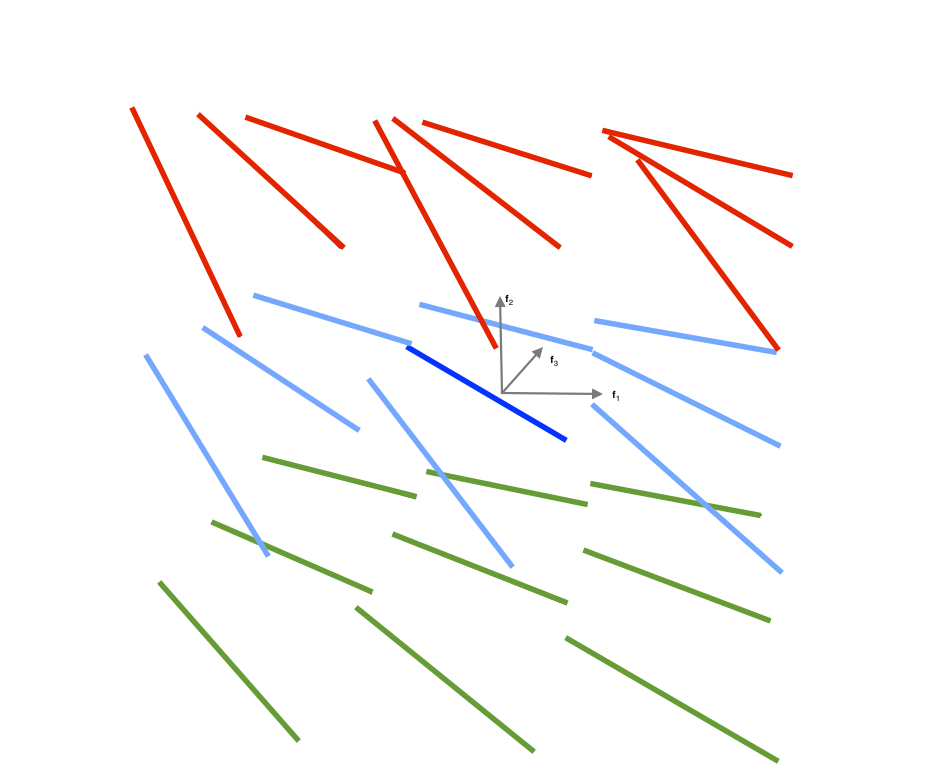
\includegraphics[width=.5\textwidth]{figures/fibers_neighborhood3d}
    \caption{Example of a fiber neighborhood of 27: the center fiber (dark blue) is where we will have a first guess for the values of the connection forms $c_{i,j,k}$ and then will run an energy minimization algorithm to come up with parameters that give the same orientation for the neighbors as we can see in the ground truth here}
    \label{fig:fibers_neighborhood3d}
\end{figure}

Finding out the correct values for the connection form parameters $c_{i,j,k}(\mathbf{x}) \forall \mathbf{x} \in \mathbb{R}^3$ is done by energy minimization within a neighborhood $\Omega$ \ref{fig:fibers_neighborhood3d}. This approach makes sense as the GHM is still dependent on the location in the heart, indeed the rate of turning will not be the same close to the apex for instance or where the heart wall is thinner.\\
Therefore the optimal parameters are defined as follows:
\begin{align*}
    c^*_{i,j,k}(\mathbf{x}) &= \text{argmin}_{c_{i,j,k}} \frac{1}{\Omega} \sum_{\mathbf{v} \in \Omega} \sum_{i = 1}^3 \epsilon_i(\mathbf{x} + \mathbf{v}) \\
    \epsilon_i(\mathbf{x} + \mathbf{v}) &= \arccos \Big( \mathbf{f}_i(\mathbf{x} + \mathbf{v}) . \mathbf{\tilde{f}}_i(\mathbf{x} + \mathbf{v}) \Big)
\end{align*}
where:
\begin{itemize}
    \item $\epsilon_i$ is the error function for each axis 
    \item $\mathbf{f}_i$ is the actual frame orientation at this location
    \item $\mathbf{\tilde{f}}_i$ is the current approximation of the frame orientation
\end{itemize}
The optimization strategy can be one of the standard well-known algorithms for these specific tasks: either Nelder-Mead \cite{press2007numerical} or BOBYQA \cite{powell2009bobyqa}.

\subsection{Combining both for a good description of heart fiber geometry}

The heart is made of elongated muscle cells called cardiomyocytes that are organized within a collagen matrix. The macroscopic shape is one of a truncated ellipsoid, while on a microscopic scale myocytes are stacked and form myofibers.\\
Work on histology has shown how cardiac myofibers wrap around the ventricules in helical curves. The ubiquitous analysis of myofiber geometry states out that the helix angle - $\theta$ or $c_{1,2,3}$ in previous sections, or the angle $\angle (\overrightarrow{\mathbf{f}^{i}_1}, \overrightarrow{\mathbf{f}^{i+1}_2})$ where $i$ is a tangent plane to the heart wall at this location - varies smoothly \ref{fig:helix_angle} with a total change \ref{fig:total_angle} of around 120° for mammals.\\
\begin{figure}[!h]
    \centering
    \begin{subfigure}[t]{.48\textwidth}
        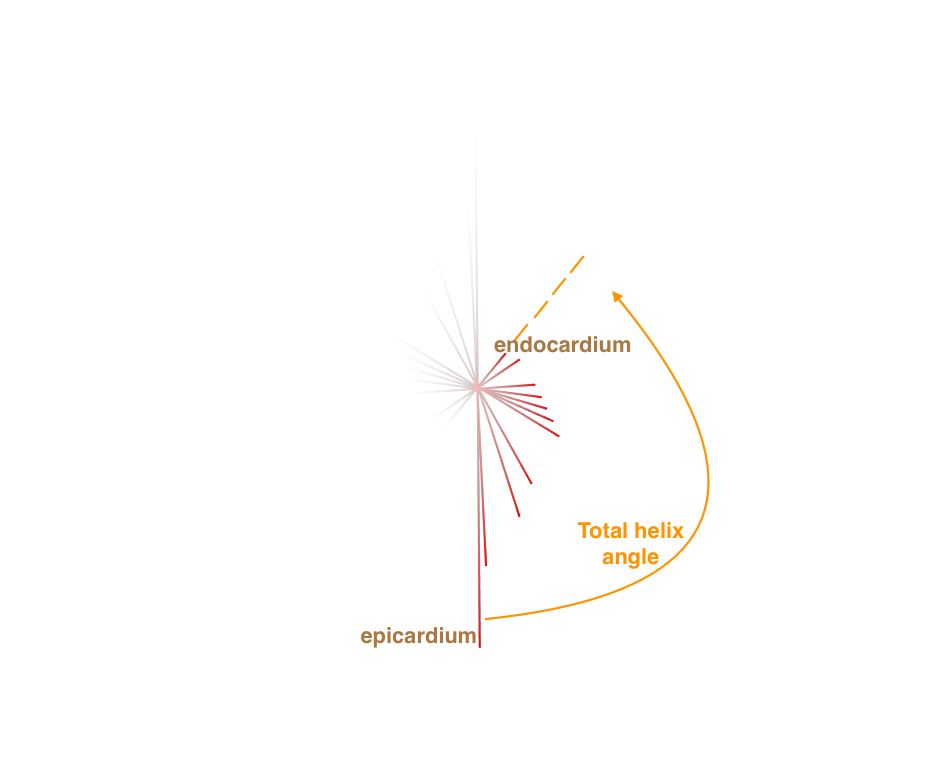
\includegraphics[width=\textwidth]{figures/total_angle}
        \caption[b]{Visualization of the helix angle with a transmural point of view}
        \label{fig:total_angle}
    \end{subfigure}
    \begin{subfigure}[t]{.48\textwidth}
        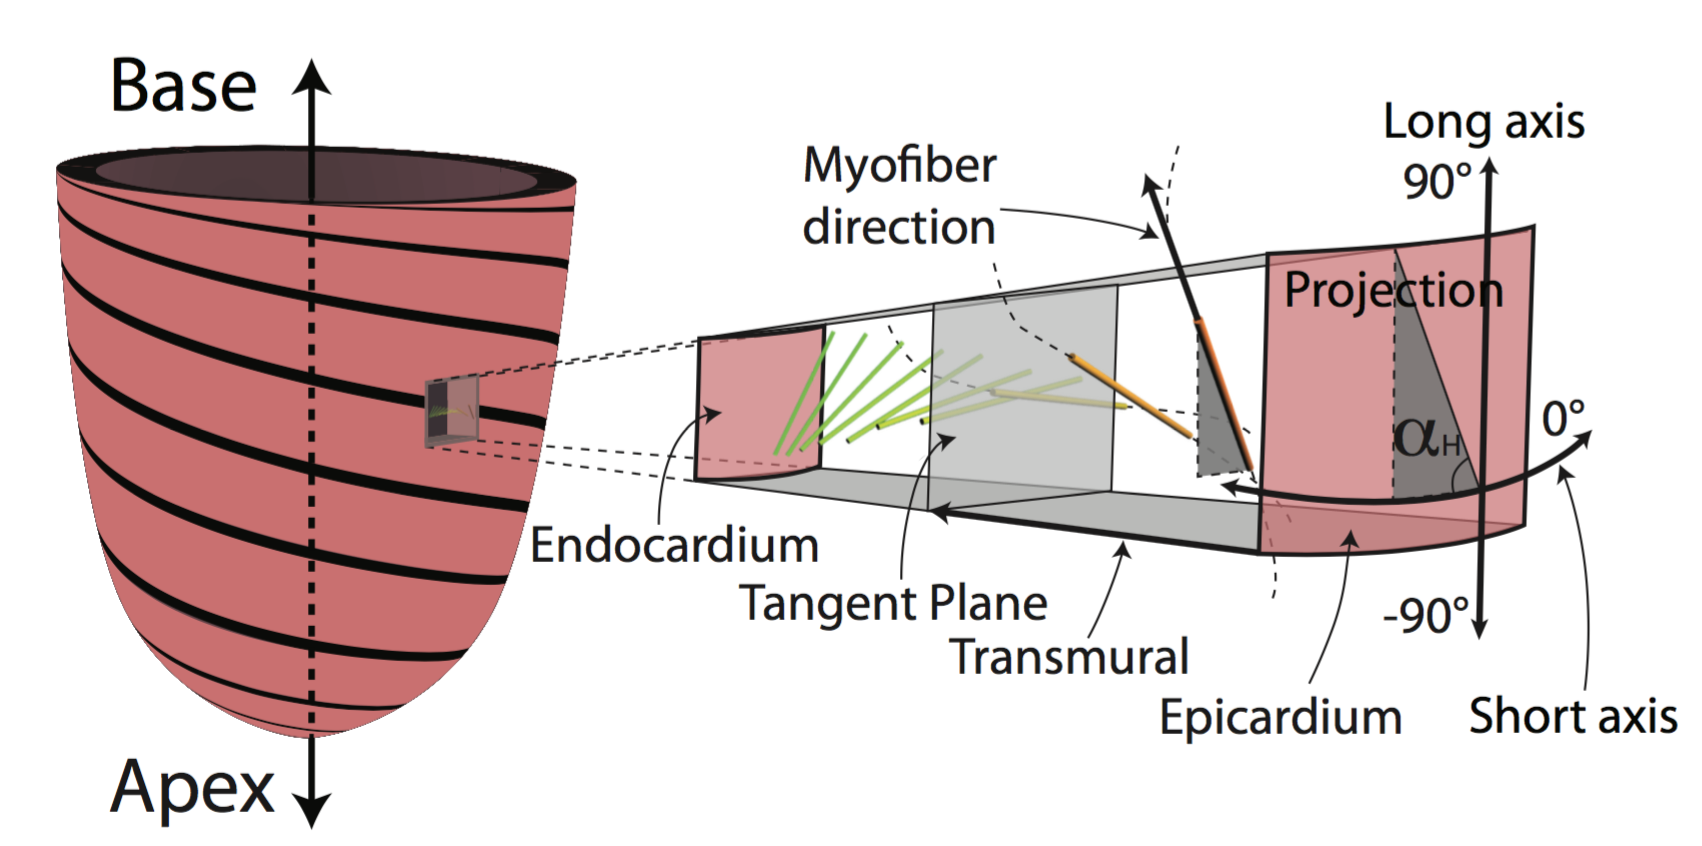
\includegraphics[width=\textwidth]{figures/helix_angle}
        \caption{The helix angle varies smoothly from one tangent plane to the other from the epicardium to the endocardium}
        \label{fig:helix_angle}
    \end{subfigure}
    \caption{Helix angle}
\end{figure}
\\
Applying this method to the heart can be done by choosing $\mathbf{f}_i$ as described previously in the GHM model. $\mathbf{f}_1$ is easy to set from the DTI data, while $\mathbf{f}_3$ is determined locally by an approximation of the transmural direction at each location using a mask of the studied heart and a euclidian distance computed between the epicardium (outtermost layer of the heart wall) and endocardium (innermost layer) of the heart.\\
The Maurer-Cartan connection form approach is a good one to describe the cardiac frame field, where the 3 main geometrical features are exhibited by parameters of this model:
\begin{itemize}
    \item $c_{1,2,3}$ for the helix angle, or trans-mural penetration of the heart wall
    \item $c_{1,3,1}$ quantifies the short-axis (in plane for a given slice) curvature of the heart wall
    \item $c_{2,3,2}$ represents the long-axis (from one slice to another) curvature
\end{itemize}
As a reminder, in general, these coefficients $c_{i,j,k}$ express the rate of turn of the frame vector $\mathbf{f}_i$ towards $\mathbf{f}_j$ when $\mathbf{x}$ moves in the direction $\mathbf{f}_k$.

\section{Infarcts and their impact on heart fiber geometry}

Studies have been trying to determine the consequences of myocardial infarctions in small (rat \cite{weisman1985global}) hearts and larger (porcine \cite{wu2007mr, mediamihaela}) hearts. In these studies it was shown that acute infarction led to a decrease in regional wall thickness and an increased radius of curvature, mostly in the border zone (BZ) - which is the zone close to the dense scar region but with a more heterogeneous nature due to the persistence of surviving blood vessels that keep on supplying oxygen to isolated cells.

\subsection{Myocardial remodeling after infarct}

After an infarct occurs, a remodeling happens in the heart, which means that the normally existing structure goes through a rearrangement process as a result of the infarct \cite{swynghedauw1999molecular}. Cardiac Remodeling (CR) is determined by the following facts:
\begin{enumerate}
    \item Adaptation process of the myocytes and collagen to new geometrical conditions
    \item Fibrosis - increased collagen concentration, due to senescence - deterioration with age, ischemia, inflammatory processes
    \item cell death as a result of fibrosis, the major marker of cardiac failure
\end{enumerate}
One of the first consequences of CR is a decrease of the wall thickness, which leads immediately to an increased volume of the Left Ventricule (LV). Another direct effet is cardiac heart hypertrophy, with a multiplication of nonmuscle cells (fibroblasts and endothelial cells) in the place of former muscle myocytes. A study on rats \cite{mccormick1994regional} showed that the hypertrophy lead to a 25\% increase of the heart mass 13 weeks after infarct.\\
Myocardial fibrosis is one of the major sign of malign issues in the CR process, which can lead to death by cardiac failure (CF) or severe arrhythmias.

\subsection{Effects of wall stress on tissue composition and geometry}

A main problem in the study of the consequences of an infarct on a mammal heart is the important cost that makes it difficult to get various data on animal heart after infarct, as there are limited means,  and was for a long time even impossible, to analyzing it in-vivo \cite{holmes1994scar}. Several experiments still have been made and the following chronological evolution of the cardiac fiber geometry emerged:
\begin{itemize}
    \item Local infarct expansion 1 week after the initial infarct, characterized by a stretch in a plane tangent to the epicardium and wall thinning.
    \item Scar shrinkage 3 weeks after infarction. The CR, even without reestablishing a contractile function as efficient as before the infarct, works around the infarct to compensate the work overload on the scar region.
    \item Alignment of myocardial collagen fibers with the direction of the greatest applied stress, which takes place during infarct healing
\end{itemize}

\subsection{Characteristics of collagen in infarcted hearts and arrangement of the surviving fibers} \label{surviving_fibers}

Studies \cite{mccormick1994regional} have shown that after infarct the whole heart mass increase by an average of 25\%. The infarcts were affecting the LV, and the difference in mass goes up to 58\% if only the LV (ventricule affected by the infarct) is considered.\\
A major impact of an infarct on the heart is on the collagen concentration that goes up significantly both in the scar tissue, the BZ which is specifically rich in fibrosis and in more distant regions. The concentration of collagen can double in the most affected regions of the heart. In general and throughout the whole heart the collagen concentration increases dramatically and is paired with more cross-linking of these cells.\\
Studies on human hearts \cite{de1990ventricular} have shown that arrhythmias and tachycardia can be caused by abnormal membrane variables and abnormal geometrical arrangement of the myocardial fibers.\\
Transmembrane potentials were taken and shown little difference between patients with ventricular tachycardia in a chronic phase of myocardial infarction and normal patients. This clearly indicates that the surviving myocardial fibers within an infarct can come back close to normal after a CR process. It has also been observed that surviving bundles in the subendocardial layers as well, and more surprisingly, as intramurally and subepicardially. These bundles of surviving myocytes showed an anisotropy similar to the papillary muscle of the heart, and therefore a similar coupling resistance, which makes sense as the activation signal propagates itself like a zigzag through the infarcted region of the heart.\\
After a transmural myocardial infarction, the outtermost epicardial muscle survives and its structure contributes greatly in the occurence of the reentry. These surviving muscle cells in the BZ of the epicardium are like a thin sheet over the infarct. The connections with other rare intramural muscle is not present very often, and this means that the impulses are only 2-dimensional as they cannot come from below, which prevents an appropriate circus movement and can lead to tachycardia \cite{ursell1985structural}.